\documentclass[conference]{IEEEtran}
\usepackage[margin=1in]{geometry}
\usepackage{cite}
\usepackage{amsmath,amssymb,amsfonts}
\usepackage{algorithmic}
\usepackage{graphicx}
\usepackage{textcomp}
\usepackage{tabstackengine}
\usepackage{xcolor}
\usepackage{subcaption}
\usepackage{cuted}

\title{A Steady State Model for the Continuous Conversion Ratio Charge Pump}
\author{Mark Lipski}
\begin{document}
	\maketitle
	\section{Abstract}
	This paper constructs a steady state model of the continuous conversion ratio charge pump architecture from first principles, incorporating incomplete charge transfer and finite switch resistance. The model is then verified using a pspice model of the circuit, and the limitations of the assumptions are discussed.
	\section{Introduction}
	The rise of IoT has driven the development of various ultra low power, low cost mobile systems. This results in a need for high efficiency, low cost power electronics.
	
	One candidate for addressing many of the needs of industry is the continuous conversion charge pump proposed in \cite{Butzen2019	}. The proposed structure has the benefit of providing a completely variable conversion ratio while maintaining high efficiencies. 

	While analytical models have been developed for charge pumps which incorporate switch resistance, \cite{Tanzawa2011}, the structure in \cite{Butzen2019} requires separate analysis. The following work proposes a steady state model that will incorporate the effects of incomplete charge transfer.
	
	The structure of the paper is as follows, first, a model of the charge pump will be generated. Next, the results of the model are compared to simulations performed using pspice. The results are then discussed, along with the validity of the assumptions.
	\section{Steady State Model}
	The circuit to be analyzed is the continuous conversion ratio circuit proposed in \cite{Butzen2019}, seen in Fig. \ref{fig:contTop}. 
	\subsection{Circuit Operation}
	The continuous conversion ratio charge pump functions substantially differently from the traditional switched capacitor power converter in its operation. Conceptually, the flying capacitors are charged by connecting the top plate to $V_{IN}$, then discharge by connecting to $V_{OUT}$, delivering current to the output.
	
	This process is made efficient using adiabatic charging methods similar to those in \cite{svensson1994}, \cite{Butzen2016}, in which capacitors are gradually charged and discharged. The charging occurs over numerous steps, where the top plate connects to intermediary voltages between $V_{OUT}$ and $V_{IN}$, labeled ($T_1$ $\rightarrow$ $T_M$), with $M$ indicating the number of intermediary levels. The bottom plate intermediary nodes are labeled $B_1$ to $B_N$.
	
	The various steps are numbered along with their associated capacitors in Fig. \ref{fig:contTop}, in steps (1,0 $\rightarrow$ 1,N) the bottom plate voltage is decreased, supplying nodes ($B_1 \rightarrow B_N$) with current. This current is then used to increase the bottom plate voltage over steps (3,1 $\rightarrow$ 3,N), simultaneously delivering current to the output. A similar process occurs with the top plate on steps (2,1 $\rightarrow$ 2,M) and (4,1 $\rightarrow$ 4,M) where current is drawn from the input.
	
	The circuit diagram corresponding to a single flying capacitor and its switches (also referred to as a "core") can be seen in Fig. \ref{fig:coreCon}. The analysis and modeling is performed under the following assumptions,
	\begin{itemize}
		\item All the capacitors are linear.
		\item The top and bottom plate parasitic capacitance's have minimal impact on the transient and steady state characteristics of the converter, and are neglected from the analysis.
		\item All the flying capacitors are equally sized with capacitance $C_{Fly}$, where $C_{Fly} = C_{1,0} = C_{1,1} = C_{2,0} = C_{2,M} ...$
		\item The input and output voltages $V_{IN}$, and $V_{OUT}$ are constant and ideal.
		\item The switches for the intermediary nodes, $S_{T1}, S_{T2}$, $S_{TM}, S_{B1}, S_{BN}, etc$, all have an equivalent resistance $R_{ON}$. The resistance of the switches which connect to the positive and negative rails ($S_{T+}, S_{T-}, S_{B+}, S_{B-}$) is 0$\,\Omega$.
	\end{itemize}
	\begin{figure}
		\centering
		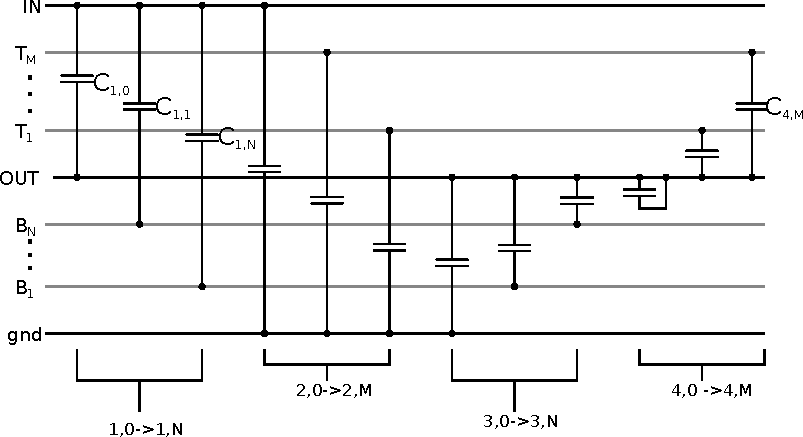
\includegraphics[width=\linewidth]{Figures/contRatioCircuit2.pdf}
		\caption{Circuit diagram illustrating the various connections made by the flying capacitors for the continuous ratio.}
		\label{fig:contTop}
	\end{figure}
	\begin{figure}
		\centering
		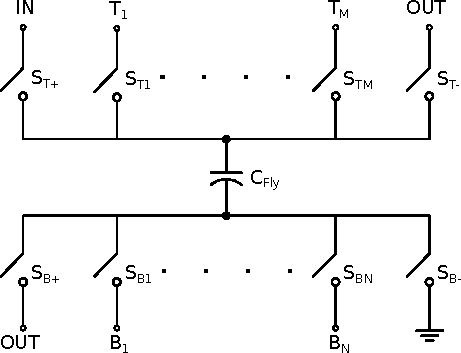
\includegraphics[width=0.6\linewidth]{Figures/contRatioCore.pdf}
		\caption{Circuit diagram illustrating the top and bottom connections of a single flying capacitor.}
		\label{fig:coreCon}
	\end{figure}
	\subsection{Charge Transfer Analysis}
	The operation of the converter involves each capacitor iterating from steps (1,0)$\rightarrow$(4,M) sequentially. There is always a connection on the top or bottom plate to either 0$\,$V, $V_{IN}$ or $V_{OUT}$. Connections to the intermediary voltage domains (those being $B_1 \rightarrow B_N$ and $T_1 \rightarrow T_M$) occur through a switch with a resistance $R_{ON}$. An example circuit can be seen in Fig. \ref{fig:step_Circ1}, which is electrically equivalent to Fig. \ref{fig:step_Circ2}. 
	
	\begin{figure}
		\centering
		\begin{subfigure}{0.45\linewidth}
			\centering
			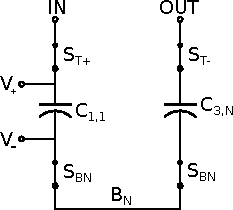
\includegraphics[width=\textwidth]{Figures/step2_Circ.pdf}
			\caption{Circuit configuration including switches and flying capacitors.}
			\label{fig:step_Circ1}
		\end{subfigure}
		\hfill
		\begin{subfigure}{0.45\linewidth}
			\centering
			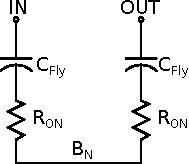
\includegraphics[width=\linewidth]{Figures/step2_Eq.pdf}
			\caption{Equivalent circuit with values.}
			\label{fig:step_Circ2}	
		\end{subfigure}
		\caption{Example circuit diagrams showing the connection to $B_N$.}
	\end{figure}

	\begin{figure}
		\centering
		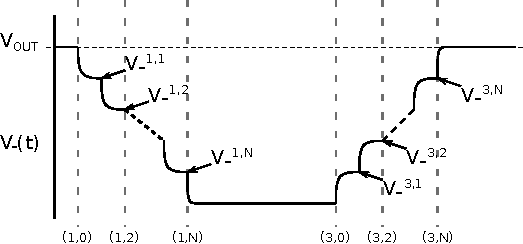
\includegraphics[width=0.9\linewidth]{Figures/V-(t).pdf}
		\caption{Illustration of $V_{-}(t)$ for various time steps over the period, where $V_-$ is the bottom plate of the capacitor, as in \ref{fig:step_Circ1}.}
		\label{fig:V-(t)}
	\end{figure}
	
	The circuit diagram in Fig. \ref{fig:step_Circ2} can be used to calculate the transient response of the circuit over each time step. Consider node $B_N$, the impedance of the branches to IN and OUT are identical, this symmetry results in $B_N$ being constant over a single time step. The top and bottom plate voltages of the capacitors can then be described using a single $RC$ time constant ($\tau$), where $\tau = R_{ON}C_{Fly}$. Using Fig. \ref{fig:step_Circ2} as an example, the top plate voltage of $C_{1,1}$ is known, while the bottom plate voltage ($V_{-}^{1,1}$) can be calculated as,
	\begin{equation}
	V_{-}^{1,1}(t) = V_{OUT}\exp\left(\frac{-t}{\tau}\right) + V_{BN}\left(1-\exp\left(\frac{-t}{\tau}\right)\right),
	\end{equation}
	where $t$ is the time after the start of the step. More generally, the top and bottom plate voltages can be described as,
	\begin{equation}
	V_{C}[n]\! =\! V_{C}[n\!-\!1]\exp\left(\tfrac{-1}{\tau f_{SW}}\right) + V_{int}\!\left(1-\exp\left(\tfrac{-t}{\tau f_{SW}}\right)\right),
	\label{eq:Vstepn}
	\end{equation}
	where $V_{C}[n-1]$ is the voltage at the end of previous step, while $V_{int}$ is the voltage of the intermediary node ($V_{T1}$, $V_{TM}$, $V_{B1}$, etc) which the capacitor is connected to. Next, the duration of each time step can be incorporated into the analysis using the switching frequency ($f_{SW}$). A substitution can then be made to simplify the analysis, where
	\begin{equation}
	A = 1-\exp\left(\tfrac{-1}{\tau f_{SW}}\right),
	\label{eq:A}
	\end{equation}
	which can be substituted into (\ref{eq:Vstepn}) resulting in
	\begin{equation}
		V_{C}[n] = V_C[n-1](1-A) + AV_{int}.
	\end{equation}
	This can be used to express the bottom plate voltage for steps (1,1)$\rightarrow $(1,N), where
	\begin{equation}
	\begin{split}
	V_-^{1,1} &= V_{OUT}(1-A) + AV_{BN},\\
	V_-^{1,2} &= V_-^{1,1}(1-A) + AV_{BN-1},\\
	& \,\,\,\vdots\\
	V_{-}^{1,N} &= V_-^{1,N-1}(1-A) + AV_{B1}.
	\end{split}		
	\end{equation}
	Using this, a matrix can be constructed to describe the bottom plate voltages,
	
	\begin{equation}
	\begin{split}
	\begin{bmatrix}
	V_-^{1,1} \\
	V_-^{1,2} \\
	\vdots\\
	V_-^{1,N-1} \\ 
	V_-^{1,N}
	\end{bmatrix}
	&\!=\!
	H\!\begin{bmatrix}
	V_{BN} \\
	V_{BN-1} \\
	\vdots \\
	V_{B2} \\
	V_{B1}
	\end{bmatrix}\!+\!V_{OUT}\!\begin{bmatrix}
	(1-A) \\
	(1-A)^2 \\
	\vdots \\
	(1\!-\!A)^{N-1} \\
	(1\!-\!A)^N
	\end{bmatrix}\!,
	\end{split}
	\label{eq:V_1}
	\end{equation}
	where,
	
	\begin{equation}
	\begin{split}
	H
	&\!=\!
	\arraycolsep2pt 
	\begin{bmatrix}
	A \!& 0 & \dots & 0 & 0 \\
	A(1-A) \!& A & \dots & 0 & 0\\
	\vdots & \vdots & \ddots & \vdots & \vdots \\
	A(1\!-\!A)^{N-2} \!& A(1\!-\!A)^{N-3} \!& \dots & A & 0\\ 
	A(1\!-\!A)^{N-1} \!& A(1\!-\!A)^{N-2} \!& \dots & A(1-A) & A 
	\end{bmatrix}.\!
	\end{split}
	\label{eq:M}
	\end{equation}
	Using a similar method, a matrix can be constructed for the bottom plate voltages in steps (3,N)$\rightarrow$(3,1).
	\begin{equation}
	\begin{split}
	\begin{bmatrix}
		V_-^{3,N} \\
		V_-^{3,N-1} \\
		\vdots\\
		V_-^{3,2} \\ 
		V_-^{3,1}
		\end{bmatrix}
		&\!=\!
		H^T\!\begin{bmatrix}
		V_{BN} \\
		V_{BN-1} \\
		\vdots \\
		V_{B2} \\
		V_{B1}
		\end{bmatrix}.
		\end{split}
		\label{eq:V_3}
		\end{equation}
	
	To calculate the values of $V_{B1}\rightarrow V_{BN}$, the amount of charge delivered to these nodes on each time step must be known. For steps, (1,1)$\rightarrow $(1,N), the charge delivered to $Bx$ is,
	\begin{equation}
	Q_{Bx} = C_{Fly}(V_-^{1,x} - V_-^{1,x-1}),
	\label{eq:Q_Bx}
	\end{equation}
	where $x$ ranges from 1 to $N$. A matrix for the charge delivered on steps $(1,1)\rightarrow(1,N)$ can then be constructed using (\ref{eq:V_1}) and (\ref{eq:Q_Bx})
	\begin{equation}
	\begin{bmatrix}
	Q_{BN} \\
	Q_{BN-1} \\
	\vdots\\
	Q_{B2} \\ 
	Q_{B1}
	\end{bmatrix}\!
	= \!
	CG\!\begin{bmatrix}
	V_{BN} \\
	V_{BN-1} \\
	\vdots \\
	V_{B2} \\
	V_{B1}
	\end{bmatrix}\!+ \!CV_{DD}\!\begin{bmatrix}
	A \\
	A(1-A) \\
	\vdots \\
	A(1\!-\!A)^{N-2} \\
	A(1\!-\!A)^{N-1}
	\end{bmatrix},
	\label{eq:Q_V1}
	\end{equation}	
	where
	\begin{equation}
	G\!=\!	
	\arraycolsep3pt 
	\begin{bmatrix}
	-A \!& 0 & \dots & 0 & 0 \\
	A^2 \!& -A & \dots & 0 & 0\\
	\vdots & \vdots & \ddots & \vdots & \vdots \\
	A^2(1\!-\!A)^{N-3} \!& A^2(1\!-\!A)^{N-4} \!& \dots & -A & 0\\ 
	A^2(1\!-\!A)^{N-2} \!& A^2(1\!-\!A)^{N-3} \!& \dots & A^2 & -A 
	\end{bmatrix}.
	\end{equation}
	
	Using a similar procedure, the charge delivered on steps $(3,1)\rightarrow(3,N)$ is,
	\begin{equation}
	\begin{bmatrix}
	Q_{BN} \\
	Q_{BN-1} \\
	\vdots\\
	Q_{B2} \\ 
	Q_{B1}
	\end{bmatrix}
	=
	C G^T
	\begin{bmatrix}
	V_{BN} \\
	V_{BN-1} \\
	\vdots \\
	V_{B2} \\
	V_{B1}
	\end{bmatrix}.
	\label{eq:Q_V3}
	\end{equation}
	The steady state condition occurs when the net charge into the intermediary nodes is 0. This can be acquired by adding (\ref{eq:Q_V1}) and (\ref{eq:Q_V3}), then equating to zero,
	
	\begin{equation}
		\begin{bmatrix}
			0 \\
			0 \\
			\vdots\\
			0 \\ 
			0
		\end{bmatrix}\!
		=
		\!(G\!+\!G^T)\!
		\begin{bmatrix}
			V_{BN} \\
			V_{BN-1} \\
			\vdots \\
			V_{B2} \\
			V_{B1}
		\end{bmatrix}\!
		+ \!V_{DD}\!\begin{bmatrix}
		A \\
		A(1-A) \\
		\vdots \\
		A(1\!-\!A)^{N-2} \\
		A(1\!-\!A)^{N-1}
	\end{bmatrix},	
	\end{equation}
	
	solving this expression for $V_{B1} \rightarrow V_{BN}$ yields,
	\begin{equation}
	V_{Bx} = V_{OUT}\frac{A(x-1) + 1}{A(N-1) + 2}.
	\end{equation}
	A similar procedure can be followed to acquire the voltage levels for $V_{T1} \rightarrow V_{TM}$,
	\begin{equation}
	V_{Ty} = V_{OUT} + (V_{IN} - V_{OUT})\frac{A(y-1) + 1}{A(M-1) + 2}\,,
	\end{equation}
	where y ranges from 1 to $M$.
	These can now be substituted into (\ref{eq:V_1}) for example to acquire the solved expressions for $V_-$ for steps (1,1) $\rightarrow$ (1,N).
	The solved expressions for the top and bottom plate voltages are:
	\begin{equation}
	V_{-}^{1,x} = \frac{((N-x-1)A + 2)V_{OUT}}{A(N-1) + 2},
	\end{equation}
	\begin{equation}
	V_{+}^{2,y} = V_{OUT} + (V_{IN} -V_{OUT})\tfrac{(M-y-1)A + 2}{A(M-1) + 2},
	\end{equation}
	\begin{equation}
	V_{-}^{3,x} = \frac{xAV_{OUT}}{A(N-1) + 2},
	\end{equation}
	\begin{equation}
	V_{+}^{4,y} = V_{OUT} + \tfrac{yA(V_{IN} -V_{OUT})}{A(M-1) + 2}.
	\end{equation}
	The charge delivered to the output can be observed from Fig. \ref{fig:contTop}, where it occurs on steps (1,0), (3,0)$\rightarrow$(3,N) and (4,1)$\rightarrow$(4,M). The charge transferred on the steps is as follows,
	\begin{equation}
	Q_{3,0} = C_{Fly}(V_+^{2,M} - V_{OUT}),
	\end{equation}
	\begin{equation}
	Q_{3,1} \rightarrow  Q_{3,N} = C_{Fly}V_{3,N},
	\end{equation}
	and
	\begin{equation}
	Q_{4,1} \rightarrow  Q_{1,0} = C_{Fly}(V_{IN} - V_{OUT}),
	\end{equation}
	resulting in a total output charge of 
	\begin{equation}
	\begin{split}
	Q_{OUT}\! &= Q_{3,0} + Q_{3,1} + Q_{4,1}\\
	Q_{OUT}\! &= \! C_{Fly}\!\left(\tfrac{(A(M-2) + 4)(V_{IN} - V_{OUT})}{A(M-1) + 2}\! + \! \tfrac{NAV_{OUT}}{A(N-1) + 2}\right).
	\end{split}
 	\end{equation}
 	A similar method can be used to acquire the input charge, occurring over steps (1,0) $\rightarrow$ (2,0),
 	\begin{equation}
 	\begin{split}
 	Q_{IN} &= C_{Fly}\left(V_{IN} - V_+^{4,M} + V_{OUT}\right) \\
 	Q_{IN} &= C_{Fly}\!\left(V_{IN} - V_{OUT} - \tfrac{MA(V_{IN}\! -\!V_{OUT})}{A(M-1) + 2} + V_{OUT}\!\right) \\
 	Q_{IN} &= C_{Fly}\tfrac{MAV_{OUT} + (2-A)V_{IN}}{A(M-1) + 2}.
 	\end{split}
 	\end{equation}
 	The input and output charge can then be used in combination with the switching frequency to acquire the input and output power,
 	\begin{equation}
 	P_{IN} = V_{IN}f_{SW}C_{Fly}\frac{MAV_{OUT} + (2-A)V_{IN}}{A(M-1) + 2},
 	\label{eq:P_IN}
 	\end{equation}
 	
 	\begin{equation}
 	\begin{split}
 	P_{OUT} &= V_{OUT}f_{SW}C_{Fly}\Big(\tfrac{(2-A)(V_{IN} - V_{OUT})}{A(M-1) + 2} \\ 
 	&+ \tfrac{NAV_{OUT}}{A(N-1) + 2} + (V_{IN} - V_{OUT})\Big).
 	\end{split} 	
 	\label{eq:P_OUT}
 	\end{equation}
 	In order to verify (\ref{eq:P_IN}) and (\ref{eq:P_OUT}), the calculations are compared to simulation data which corresponded to the prior assumptions. The simulation results were acquired using pspice, in which 36 of the cores in Fig. \ref{fig:coreCon} were used to simulate an N = M = 8 use case. Additional variables used in the simulations were $V_{OUT}$ = 2.5$\,$V, $f_{SW}$ = 250$\,$MHz, $C_{Fly}$ = 1$\,$nF, and $R_{ON}$ was swept between 0.1$\Omega$ and 4$\Omega$. The resulting comparison is graphed in Fig. \ref{fig:Comp_A}, with an average error of $<$0.3\% in both $P_{IN}$ and $P_{OUT}$.
 	
 	\begin{figure}
 		\centering
 		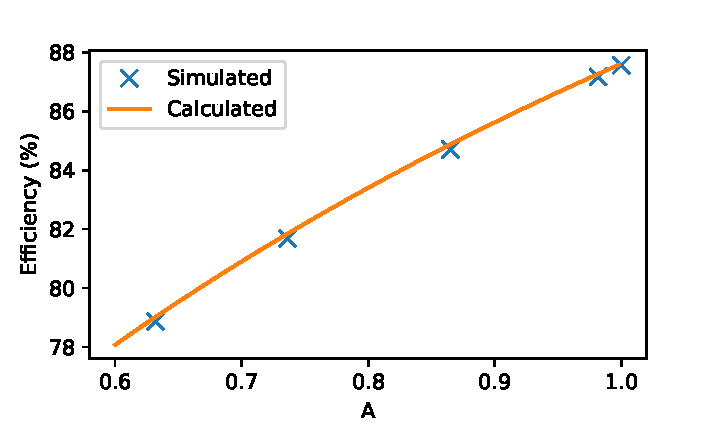
\includegraphics[width=\linewidth]{Figures/eta_A.pdf}
 		\caption{Comparison between calculated and simulated efficiency results for various values of A and $V_{IN}$.}
 		\label{fig:Comp_A}
 	\end{figure}
 	\subsection{Incorporating Transistor Switching Losses}
 	The power lost switching the gates of the transistors on and off can either be added to $P_{IN}$, or subtracted from $P_{OUT}$, depending on the bootstrapping and control method used. The power can be calculated using $f_{SW}$, along with the total gate capacitance of all the switches ($C_{G}$), and the switching voltage ($V_{SW}$),
 	\begin{equation}
 	P_{SW} = f_{SW}V_{SW}^2C_G.
 	\end{equation}
 	This will allow the designer to fully calculate the design trade-off associated with transistor sizing. 
 	
 	
 	\section{Steady State Model Usefulness}
 	The usefulness of the model is going to be dependent on how accurate the underlying assumptions are, these will now be discussed. 
 	\subsection{Switch Resistance}
 	The fixed, time invariant on-resistance of the transistors is an approximation, however the relative bias structure used in \cite{Butzen2019} should eliminate the variation in $R_{ON}$ based on the top and bottom plate voltages.
 	
 	The next portion of this assumption is that switches $S_{B+}$, $S_{B-}$, $S_{T+}$ and $S_{T-}$ have a resistance of 0$\,\Omega$. The reality is that these switches should be sized a factor $\sqrt{M+1}$ or $\sqrt{N+1}$ larger than the other transistors in order to minimize both capacitive and resistive losses. The designer then only needs to incorporate this resistance into (\ref{eq:A}), 
 	\begin{equation}
 	A = 1-\exp\left(\tfrac{-1}{C_{Fly}R_{ON}(1+\sqrt{M+1}) f_{SW}}\right),
 	\end{equation}
 	which will approximate the resulting impact on performance.
 	\subsection{Constant $V_{IN}$ and $V_{OUT}$}
 	This assumption is going to depend entirely on the filtering capacitors used at the input and output. Realistically, there is going to be a reduction in the efficiency resulting from ripple in the input and output. This can be reduced by adapting the out-phasing technique used in \cite{Le2010} to the circuit.
 	
 	\section{Discussion}
 	The proposed model is useful for giving an approximation of the efficiency, and predicting its relationship with the switch resistance. This can be used to optimize transistor sizing, along with selecting $N$ and $M$. There exists a further need to incorporate additional effects into the model, such as transistor leakage effects, and exploring the exact impact of non-linearities on the performance of the configuration. 
 	
 	Finally, the model would benefit from further verification by incorporating post layout transistor models, as well as verifying the model using a fabricated device.
 	
 	\section{Conclusion}
 	In this paper, a steady state model of the continuous ratio charge pump architecture is presented. The model is then verified using pspice simulations, which results in a prediction of the input and output power to $<$0.3\% average error. The results and limitations of the model are then discussed.
 	
 	\bibliographystyle{IEEEtran}
 	\bibliography{contBib}
\end{document}